\chapter{多维随机变量及其分布}
\section{二维随机变量及其分布函数}
\subsection{二维随机变量及其分布函数}
\begin{definition}
设\(X\)与\(Y\)是定义在同一样本空间\(\Omega\)上的两个随机变量,%
则称\((X,Y)\)为二维\textbf{随机变量}(或\textbf{随机向量}).
\end{definition}

\begin{definition}
设\((X,Y)\)是二维随机变量,对任意实数\(x\),\(y\),称\begin{equation}\label{equation:多维随机变量及其分布.二维分布函数的定义式}
F(x,y) = P(X \leqslant x, Y \leqslant y)
\end{equation}为二维随机变量\((X,Y)\)的\textbf{二维分布函数},%
或称之为\(X\)与\(Y\)的\textbf{联合分布函数}.
\end{definition}

\begin{property}
\(P(x_1 < X \leqslant x_2, y_1 < Y \leqslant y_2)
= F(x_2,y_2) - F(x_2,y_1) - F(x_1,y_2) + F(x_1,y_1)\).
\end{property}

\begin{property}
设\(F(x,y)\)为随机变量\((X,Y)\)的分布函数,则
\begin{enumerate}
\item \(F(x,y)\)分别关于\(x\)及\(y\)单调不减,即
当\(x_1 < x_2\)时,有\(F(x_1,y) \leqslant F(x_2,y)\);
当\(y_1 < y_2\)时,有\(F(x,y_1) \leqslant F(x,y_2)\).
\item \(F(-\infty,-\infty)=F(-\infty,y)=F(x,-\infty)=0\),\(F(+\infty,+\infty)=1\).
\item \(F(x,y)\)关于\(x\)及\(y\)都右连续,即对任意实数\(x\)、\(y\)有
\(F(x^+,y)=F(x,y)\)和\(F(x,y^+)=F(x,y)\)成立.
\item 对任意\(x_1 < x_2\)、\(y_1 < y_2\)有\[
P(x_1 < X \leqslant x_2, y_1 < Y \leqslant y_2)
= F(x_2,y_2) - F(x_2,y_1) - F(x_1,y_2) + F(x_1,y_1)
\geqslant 0.
\]
\end{enumerate}
\rm
需要指出,上述四点也是二维分布函数的特征,即任何一个二元函数只要满足这四点就是某二维随机变量的分布函数.
\end{property}

\section{二维离散型随机变量及其概率分布}

\subsection{二维离散型随机变量及其概率分布的概念与性质}
\begin{definition}
如果二维随机变量\((X,Y)\)只取有限个或可数无穷个点对\((x_i,y_i)\ (i,j=1,2,\dotsc)\),%
则称\((X,Y)\)为\textbf{二维离散型随机变量}.
\end{definition}

\begin{definition}
设二维离散型随机变量\((X,Y)\)所有可能取值为\((x_i,y_i)\ (i,j=1,2,\dotsc)\),记\[
p_{ij} = P(X = x_i, Y = y_j), \quad i,j = 1,2,\dotsc,
\]则称上式为\((X,Y)\)的\textbf{二维概率分布}或\textbf{二维概率分布律},%
或称为\(X\)与\(Y\)的\textbf{联合概率分布}.
\end{definition}

二维概率分布可以用\cref{table:多维随机变量及其分布.二维概率分布} 表示.

\begin{table}[ht]
\centering
\begin{tabular}{c|*5c}
	& \(y_1\) & \(y_2\) & \(\dots\) & \(y_j\) & \(\dots\) \\ \hline
\(x_1\) & \(p_{11}\) & \(p_{12}\) & \(\dots\) & \(p_{1j}\) \\
\(x_2\) & \(p_{21}\) & \(p_{22}\) & \(\dots\) & \(p_{2j}\) \\
\(\vdots\) & \(\vdots\) & \(\vdots\) & & \(\vdots\) \\
\(x_i\) & \(p_{i1}\) & \(p_{i2}\) & \(\dots\) & \(p_{ij}\) \\
\(\vdots\) & \(\vdots\) & \(\vdots\) & & \(\vdots\) \\
\end{tabular}
\caption{\((X,Y)\)的二维概率分布}
\label{table:多维随机变量及其分布.二维概率分布}
\end{table}

\begin{property}
二维离散型随机变量的概率分布有如下的性质:
\begin{enumerate}
\item 非负性:\(p_{ij} \geqslant 0, \quad i,j=1,2,\dotsc\);
\item 规范性:\(\sum_{i,j} p_{ij} = 1\).
\end{enumerate}
\end{property}

\begin{theorem}
对于任意一个二维点集\(G\),对任意二维离散型随机变量\((X,Y)\)可以求事件\(((X,Y) \in G)\)的概率,即\[
P\left[(X,Y) \in G\right] = \sum_{(x_i,y_j) \in G} p_{ij}.
\]

特别地,二维离散型随机变量\((X,Y)\)的二维分布函数可用概率分布求出,即\[
F(x,y) = \sum_{x_i \leqslant x}\sum_{y_j \leqslant y} p_{ij},
\]且有\[
p_{ij} = F(x_i,y_j) - F(x_i,y_{j-1}) - F(x_{i-1},y_j) + F(x_{i-1},y_{j-1}), \quad i,j = 1,2,\dotsc,
\]其中,规定\(x_0 = y_0 = -\infty\).
\end{theorem}

\subsection{重要的二维离散型分布 —— 三项分布}
\begin{definition}
在\(n\)重独立试验中,若每次试验只有\(A_1\)、\(A_2\)、\(A_3\)三个可能结果,%
且\(0 < p_i = P(A_i) < 1\)(\(i=1,2,3\)),则\(p_1 + p_2 + p_3 = 1\).
令随机变量\(X\)及\(Y\)分别表示\(n\)次试验中\(A_1\)与\(A_2\)发生的次数,%
则\(X\)与\(Y\)的联合概率分布为\[
P(X=k_1,Y=k_2) = \frac{n!}{k_1! k_2! (n-k_1-k_2)!} p_1^{k_1} p_2^{k_2} p_3^{n-k_1-k_2},
\]其中\(k_1+k_2 = 0,1,\dotsc,n\),\(k_1 \geqslant 0\),\(k_2 \geqslant 0\),%
并称\((X,Y)\)服从参数为\(p _1\)、\(p_2\)、\(n\)的\textbf{三项分布},记为\((X,Y) \sim T(n;p_1,p_2)\).
\end{definition}

\section{二维连续型随机变量及其密度函数}

\subsection{二维连续型随机变量及其密度函数的概念与性质}

\begin{definition}
设二维随机变量\((X,Y)\)有分布函数\(F(x,y)\),如果存在二元非负函数\(f(x,y)\),使得对任意实数\(x\)、\(y\)有\[
F(x,y) = \int_{-\infty}^x \int_{-\infty}^y f(u,v) \dd{u} \dd{v},
\]则称\((X,Y)\)是\textbf{二维连续型随机变量},称\(f(x,y)\)为\((X,Y)\)的\textbf{二维概率密度函数},%
或称为\(X\)与\(Y\)的\textbf{联合密度函数},简称为\textbf{密度函数}或\textbf{密度}.
\end{definition}

\begin{property}
二维连续型随机变量的密度函数有如下的性质:
\begin{enumerate}
\item \(f(x,y) \geqslant 0\ (x,y)\in\mathbb{R}^2\);
\item \(F(+\infty,+\infty) = \int_{-\infty}^{+\infty} \int_{-\infty}^{+\infty} f(x,y) \dd{x} \dd{y} = 1\).
\end{enumerate}
\end{property}

\begin{theorem}
设二维连续型随机变量\((X,Y)\)有密度函数\(f(x,y)\),则
\begin{enumerate}
\item \(F(x,y)\)是连续函数且在\(f(x,y)\)的连续点\((x,y)\),有\[
f(x,y) = \pdv{F(x,y)}{x}{y};
\]
\item 对平面上任意区域\(G \subseteq \mathbb{R}^2\),若\(f(x,y)\)在\(G\)上可积,有\[
P\left[(X,Y) \in G\right] = \iint\limits_G{f(x,y) \dd{x}\dd{y}};
\]
\item 对平面上任一条曲线\(L\),有\[
P\left[(X,Y) \in L\right] = 0.
\]
\end{enumerate}
\end{theorem}

\subsection{重要的二维连续型分布 —— 均匀分布}
\begin{definition}
令\(G\)是平面上一个有界区域,若二维随机变量\((X,Y)\)有密度函数\[
f(x,y) = \left\{ \begin{array}{ll}
\frac{1}{m(G)}, & (x,y) \in G, \\
0, & \text{其他}, \\
\end{array} \right.
\]其中\(m(G)\)为\(G\)的面积,则称\((X,Y)\)为在\(G\)上的\textbf{均匀分布},记为\((X,Y) \sim U(G)\).
\end{definition}

\section{边缘分布及随机变量的独立性}
\subsection{边缘分布函数与随机变量的独立性}
\begin{definition}
二维随机变量\((X,Y)\)的分量\(X\)、\(Y\)均可看作一维随机变量.
这两个分量各自的分布函数\(F_X(x)\)、\(F_Y(y)\),%
相对于二维分布函数\(F(x,y)\)而被分别称为\(X\)与\(Y\)的\textbf{边缘分布函数}.
\end{definition}

\begin{theorem}
设\(F(x,y)\)为二维随机变量\((X,Y)\)的二维分布函数,%
则\(X\)与\(Y\)的边缘分布函数\(F_X(x)\)、\(F_Y(y)\)有
\begin{align*}
F_X(x) &= F(x,+\infty), \quad x \in \mathbb{R}; \\
F_Y(y) &= F(+\infty,y), \quad y \in \mathbb{R}.
\end{align*}
\end{theorem}

\begin{definition}
\(F(x,y)\)是二维随机变量\((X,Y)\)的二维分布函数,\(F_X(x)\)、\(F_Y(y)\)分别为\(X\)、\(Y\)的边缘分布函数.
若对任意\(x\)、\(y\)有\[
F(x,y) = F_X(x) F_Y(y),
\]则称“\(X\)与\(Y\)\textbf{相互独立}”.
\end{definition}

\begin{theorem}
设随机变量\(X\)与\(Y\)相互独立,且\(g(x)\)与\(h(y)\)均是连续函数,%
则\(X_1 = g(X)\)与\(Y_1 = h(Y)\)也相互独立.
\end{theorem}

\subsection{二维离散型随机变量的边缘分布及独立性}
\begin{definition}
设\((X,Y)\)是二维离散型随机变量,有二维概率分布\[
p_{ij} = P(X=x_i,Y=y_j), \quad i,j=1,2,\dotsc.
\]显然此时\(X\)与\(Y\)都是一维离散型随机变量,各有分布律
\begin{align*}
p_{i*} &= P(X=x_i), \quad i=1,2,\dotsc; \\
p_{*j} &= P(Y=y_j), \quad j=1,2,\dotsc.
\end{align*}
相对于二维概率分布,\(X\)与\(Y\)各自的分布叫做\textbf{边缘概率分布},简称\textbf{边缘分布}.
\end{definition}

\begin{theorem}
设\((X,Y)\)是二维离散型随机变量,有二维概率分布\[
p_{ij} = P(X=x_i,Y=y_j), \quad i,j=1,2,\dotsc.
\]分量\(X\)与\(Y\)的边缘分布可由二维概率分布求出,即
\begin{align*}
p_{i*} = \sum_{j}{p_{ij}}, \quad i=1,2,\dotsc; \\
p_{*j} = \sum_{i}{p_{ij}}, \quad j=1,2,\dotsc.
\end{align*}
\end{theorem}

\begin{theorem}
设\((X,Y)\)是二维离散型随机变量,有二维概率分布\[
p_{ij} = P(X=x_i,Y=y_j), \quad i,j=1,2,\dotsc,
\]则随机变量\(X\)与\(Y\)相互独立的充要条件是:\[
p_{ij} = p_{i*} p_{*j}, \quad i,j=1,2,\dotsc.
\]
\end{theorem}

\subsection{二维连续型随机变量的边缘密度及独立性}
\begin{theorem}
设二维连续型随机变量\((X,Y)\)的二维密度为\(f(x,y)\),%
\(X\)与\(Y\)的边缘密度分别为\(f_X(x)\)和\(f_Y(y)\),则
\begin{align*}
f_X(x) = \int_{-\infty}^{+\infty} f(x,y) \dd{y}, \\
f_Y(y) = \int_{-\infty}^{+\infty} f(x,y) \dd{x}.
\end{align*}

而\(X\)与\(Y\)相互独立的充要条件是:\[
f(x,y) = f_X(x) f_Y(y).
\]在三个密度函数的公共连续点上成立.
\end{theorem}

\section{条件分布与条件密度}
\subsection{离散型随机变量的条件分布}
\begin{definition}
对于任意\(y_j\),若\(P(Y=y_j) = p_{*j} > 0\),称\[
P(X=x_i \vert Y=y_j) = \frac{p_{ij}}{p_{*j}}, \quad i=1,2,\dotsc
\]为\(Y=y_j\)条件下\(X\)的\textbf{条件概率分布}.

同理,对于任意\(x_i\),若\(P(X=x_i) = p_{i*} > 0\),称\[
P(Y=y_j \vert X=x_i) = \frac{p_{ij}}{p_{i*}}, \quad j=1,2,\dotsc
\]为\(X=x_i\)条件下\(Y\)的\textbf{条件概率分布}.
\end{definition}

\begin{property}
离散型随机变量的条件概率分布有如下性质:
\begin{enumerate}
\item \(P(X=x_i \vert Y=y_j) \geqslant 0, \quad i=1,2,\dotsc;\)
\item \(\sum_{i}{P(X=x_i \vert Y=y_j)} = \sum_{i}{\frac{p_{ij}}{p_{*j}}} = 1.\)
\end{enumerate}
可见,条件概率分布也是离散型概率分布.
\end{property}

\begin{theorem}
对任意\(x\)、\(y\),由条件分布可得条件分布函数的表示:
\begin{align*}
F_{X \vert Y}(x \vert y_j) = P(X \leqslant x \vert Y=y_j) = \sum_{x_i \leqslant x}{\frac{p_{ij}}{p_{*j}}}, \\
F_{Y \vert X}(y \vert x_i) = P(Y \leqslant y \vert X=x_i) = \sum_{y_j \leqslant y}{\frac{p_{ij}}{p_{i*}}}.
\end{align*}
\end{theorem}

\subsection{连续型随机变量的条件密度函数}
\begin{definition}
设\((X,Y)\)为二维连续型随机变量.若对任意\(\varepsilon > 0\),有\[
P(y - \varepsilon < Y \leqslant y + \varepsilon) > 0,
\]且对\(x\in\mathbb{R}\),极限\[
\lim\limits_{\varepsilon\to0^+} P(X \leqslant x \vert y - \varepsilon < Y \leqslant y + \varepsilon)
\]存在,%
则称该极限为“连续型随机变量\(Y=y\)条件下\(X\)的\textbf{条件分布函数}”,%
记为\(F_{X \vert Y}(x \vert y)\)或\(P(X \leqslant x \vert Y = y)\).

类似地,可以定义%
“连续型随机变量\(X=x\)条件下\(Y\)的\textbf{条件分布函数}”%
\(F_{Y \vert X}(y \vert x)\)或\(P(Y \leqslant y \vert X = x)\).
\end{definition}

\begin{theorem}
设二维连续型随机变量\((X,Y)\)有二维密度\(f(x,y)\),%
从而\(X\)及\(Y\)有边缘密度\(f_X(x)\)、\(f_Y(y)\),则
\begin{align*}
F_{X \vert Y}(x \vert y) = \int_{-\infty}^{x} \frac{f(u,y)}{f_Y(y)}\dd{u}, \quad x \in \mathbb{R}; \\
F_{Y \vert X}(y \vert x) = \int_{-\infty}^{y} \frac{f(x,v)}{f_X(x)}\dd{v}, \quad y \in \mathbb{R}.
\end{align*}

那么,相应的密度函数
\begin{gather}
f_{X \vert Y}(x \vert y) = \frac{f(x,y)}{f_Y(y)}, \label{equation:多维随机变量及其分布.条件密度、联合密度、边缘密度的关系1} \\
f_{Y \vert X}(y \vert x) = \frac{f(x,y)}{f_X(x)}, \label{equation:多维随机变量及其分布.条件密度、联合密度、边缘密度的关系2}
\end{gather}
分别称为“\(X\)关于\(Y\)的\textbf{条件密度函数}”%
和“\(Y\)关于\(X\)的\textbf{条件密度函数}”.
\begin{proof}
不妨设\(f(x,y)\)连续,\(f_Y(y)\)连续且\(f_Y(y)>0\),%
\def\l{\lim\limits_{\varepsilon\to0^+}}%
那么\begin{align*}
F_{X \vert Y}(x \vert y)
&= \l \frac{P(X \leqslant x, y - \varepsilon < Y \leqslant y + \varepsilon)}{P(y - \varepsilon < Y \leqslant y + \varepsilon)} \\
&= \l \frac{F(x,y+\varepsilon) - F(x,y-\varepsilon)}{F_Y(y+\varepsilon) - F_Y(y-\varepsilon)} \\
&= \l \frac{[F(x,y+\varepsilon) - F(x,y-\varepsilon)] \frac{1}{2 \varepsilon}}{[F_Y(y+\varepsilon) - F_Y(y-\varepsilon)] \frac{1}{2 \varepsilon}} \\
&= \pdv{F(x,y)}{y} \bigg/ F_Y'(y)
= \int_{-\infty}^x \frac{f(u,y)}{f_Y(y)} \dd{u}.
\qedhere
\end{align*}
\end{proof}
\end{theorem}

\begin{corollary}
已知边缘密度函数和条件密度函数,可以求出二维密度,即\[
f(x,y) = f_Y(y) \cdot f_{X \vert Y}(x \vert y)
= f_X(x) \cdot f_{Y \vert X}(y \vert x).
\]
\end{corollary}

\begin{example}
设\(X \sim U(0,1)\);对\(\forall x\in(0,1)\),当\(X=x\)时,\(Y \sim U(x^2,1)\),求\(P(X > Y)\).
\begin{solution}
\(X\)的密度函数为\[
f_X(x) = \left\{ \begin{array}{cl}
1, & 0<x<1, \\
0, & \text{其他}.
\end{array} \right.
\]当\(X=x\in(0,1)\)时,\(Y\)有条件密度\[
f_{Y \vert X}(y \vert x)
= \left\{ \begin{array}{cl}
\frac{1}{1-x^2}, & x^2<y<1, \\
0, & \text{其他}.
\end{array} \right.
\]因此\[
f(x,y) = f_X(x) \cdot f_{Y \vert X}(y \vert x)
= \left\{ \begin{array}{cl}
\frac{1}{1-x^2}, & 0<x<1 \land x^2<y<1, \\
0, & \text{其他}.
\end{array} \right.
\]\[
P(X > Y)
= \int_0^1 \dd{x} \int_{x^2}^x \frac{1}{1-x^2} \dd{y}
= 1 - \ln2.
\]
\end{solution}
\end{example}

\section{二维随机变量函数的分布}
\subsection{二维离散型随机变量函数的分布}
设\((X,Y)\)是二维离散型随机变量,且\(X\)与\(Y\)有联合分布律\[
p_{ij} = P(X=x_i,Y=y_j), \quad i,j=1,2,\dotsc,
\]则\(Z = g(X,Y)\)有分布律\[
P(Z=z_k) = \sum_{g(x_i,y_j)=z_k}{p_{ij}}.
\]

\begin{example}
设\((X,Y)\)有二维概率分布
\begin{center}
\begin{tikzpicture}
	\draw[thick](0,0)--(4,0) (0,-4)--+(4,0);
	\draw(0,-1)--+(4,0) (1,0)--+(0,-4);
	\draw(1.5,-.5)node{0}
		(2.5,-.5)node{1}
		(3.5,-.5)node{2}
		(.5,-1.5)node{-1}
		(.5,-2.5)node{0}
		(.5,-3.5)node{1}
		(.3,-.7)node{\(X\)}
		(.7,-.3)node{\(Y\)}
		(1.5,-1.5)node{\(\tfrac{1}{12}\)}
		(2.5,-1.5)node{\(\tfrac{2}{12}\)}
		(3.5,-1.5)node{\(\tfrac{2}{12}\)}
		(1.5,-2.5)node{\(\tfrac{1}{12}\)}
		(2.5,-2.5)node{\(\tfrac{1}{12}\)}
		(3.5,-2.5)node{\(0\)}
		(1.5,-3.5)node{\(\tfrac{2}{12}\)}
		(2.5,-3.5)node{\(\tfrac{1}{12}\)}
		(3.5,-3.5)node{\(\tfrac{2}{12}\)};
\end{tikzpicture}
\end{center}
\(Z=X+Y\),\(W=\max\{X,Y\}\),求\(Z,W\)的分布律.
\begin{solution}
我们可以根据上面的二维概率分布表格计算不同\(X,Y\)取值下\(Z\)的取值:
\begin{center}
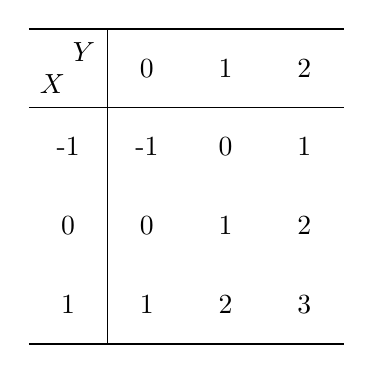
\begin{tikzpicture}
	\draw[thick](0,0)--(4,0) (0,-4)--+(4,0);
	\draw(0,-1)--+(4,0) (1,0)--+(0,-4);
	\draw(1.5,-.5)node{0}
		(2.5,-.5)node{1}
		(3.5,-.5)node{2}
		(.5,-1.5)node{-1}
		(.5,-2.5)node{0}
		(.5,-3.5)node{1}
		(.3,-.7)node{\(X\)}
		(.7,-.3)node{\(Y\)}
		(1.5,-1.5)node{-1}
		(2.5,-1.5)node{0}
		(3.5,-1.5)node{1}
		(1.5,-2.5)node{0}
		(2.5,-2.5)node{1}
		(3.5,-2.5)node{2}
		(1.5,-3.5)node{1}
		(2.5,-3.5)node{2}
		(3.5,-3.5)node{3};
\end{tikzpicture}
\end{center}
由此可知\(Z \in \Set{-1,0,1,2,3}\),那么
\def\sp#1{\sum\limits_{x_i+y_j=#1} p_{ij}}
\begin{align*}
	&P(Z=-1) = \sp{-1} = \frac{1}{12}, \\
	&P(Z=0) = \sp{0} = \frac{1}{4}, \\
	&P(Z=1) = \sp{1} = \frac{5}{12}, \\
	&P(Z=2) = \sp{2} = \frac{1}{12}, \\
	&P(Z=3) = \sp{3} = \frac{1}{6},
\end{align*}
即\[
	Z \sim \begin{bmatrix}
		-1 & 0 & 1 & 2 & 3 \\
		\frac{1}{12} & \frac{1}{4} & \frac{5}{12} & \frac{1}{12} & \frac{1}{6}
	\end{bmatrix}.
\]
同理可得,\[
	W \sim \begin{bmatrix}
		0 & 1 & 2 \\
		\frac{1}{6} & \frac{1}{2} & \frac{1}{3}
	\end{bmatrix}.
\]
\end{solution}
\end{example}

\subsection{二维连续型随机变量函数的分布}
设\((X,Y)\)是二维连续型随机变量,且有密度函数\(f(x,y)\).
若\(g(x,y)\)是连续函数,则\(Z = g(X,Y)\)是一维连续型随机变量.
\begin{enumerate}
\item 首先确定\(Z\)的值域\(R(Z)\);
\item 对任意\(z \in R(Z)\),求\(Z\)的分布函数\(F_Z(z)\),即\begin{align*}
F_Z(z) &= P(Z \leqslant z)
= P[g(X,Y) \leqslant z]
= P[(X,Y) \in G(z)] \\
&= \iint_{G(z)} f(x,y) \dd{x}\dd{y}.
\end{align*}
这里\(G(z) = \Set{ z\in\mathbb{R} \given g(x,y) \leqslant z }\).
当\(z \notin R(Z)\)时,有\(F_Z(z)=0\)或\(F_Z(z)=1\).
\item 求导得到\(Z\)的密度函数\(f_Z(z) = F'_Z(z)\).
\end{enumerate}

\begin{example}
设\((X,Y)\)的密度函数为\[
f(x,y) = \left\{ \begin{array}{cl}
xy, & 0 \leqslant x \leqslant 2, 0 \leqslant y \leqslant 1, \\
0, & \text{其他}.
\end{array} \right.
\]求\(Z = XY\)的密度.
\begin{solution}
\begin{figure}[ht]
	\centering
	\begin{tikzpicture}
		\begin{scope}[>=Stealth,->]
			\draw(0,0)node[below left]{\(O\)}--(3,0)node[below]{\(x\)};
			\draw(0,0)--(0,2)node[left]{\(y\)};
		\end{scope}
		\draw(0,1)node[left]{\(1\)}--(2,1)--(2,0)node[below]{\(2\)};
		\pgfmathsetmacro{\z}{1.5}
		\pgfmathsetmacro{\y}{\z/2}
		\draw[dashed](\z,0)node[below]{\(z\)}--(\z,1)node[above right]{\(xy=z\)};
		\pgfmathsetmacro{\a}{3*(2+\z)/4}
		\pgfmathsetmacro{\r}{.5*sqrt(2.5)*sqrt(4+\z^2)}
		\pgfmathsetmacro{\sx}{.8}
		\pgfmathsetmacro{\sy}{\a-sqrt(\r^2-(\sx-\a)^2)}
		\pgfmathsetmacro{\dx}{2.5}
		\pgfmathsetmacro{\dy}{\a-sqrt(\r^2-(\dx-\a)^2)}
		\draw(\sx,\sy)..controls(\z,.85)..(\dx,\dy);
	\end{tikzpicture}
	\caption{}
	\label{figure:多维随机变量及其分布.二维连续型随机变量函数的分布.例1}
\end{figure}
由题意有,\(Z\)的值域为\(R(Z)=[0,2]\).
如\cref{figure:多维随机变量及其分布.二维连续型随机变量函数的分布.例1},
对\(\forall z\in[0,2]\),有\begin{align*}
	F_Z(z) &= P(Z \leqslant z)
	= P(XY \leqslant z)
	= \iint_{xy \leqslant z} f(x,y) \dd{x}\dd{y} \\
	&= \int_0^z \dd{x} \int_0^1 xy \dd{y}
		+ \int_z^2 \dd{x} \int_0^{z/x} xy \dd{y} \\
	&= \frac{z^2}{4} + \frac{z^2}{2} (\ln2 - \ln z),
\end{align*}
于是\[
	f_Z(z) = F_Z'(z)
	= \left\{ \begin{array}{cl}
		z \ln(2/z), & 0<z\leqslant2, \\
		0, & \text{其他}.
	\end{array} \right.
\]
\end{solution}
\end{example}

\begin{example}
设\(X \sim U(0,1)\),\(Y \sim e(1)\),且\(X\)与\(Y\)相互独立,\(Z = X+Y\).
求\(Z\)的密度函数.
\begin{solution}
由题意有,\((X,Y)\)的密度函数为\[
	f(x,y) = \begin{cases}
		e^{-y}, & 0<x<1,y>0, \\
		0, & \text{其他};
	\end{cases}
\]
\(Z\)的值域为\(R(Z)=(0,+\infty)\).
对\(\forall z>0\),有\begin{align*}
	F_Z(z) &= P(Z \leqslant z) = P(X+Y \leqslant z) \\
	&= \iint_{x+y \leqslant z} f(x,y) \dd{x}\dd{y}.
\end{align*}
\begin{figure}
	\centering
	\begin{tikzpicture}
		\begin{scope}[>=Stealth,->]
		\draw(0,0)node[below left]{\(O\)}--(4,0)node[below]{\(x\)};
		\draw(0,0)--(0,4)node[left]{\(y\)};
		\end{scope}
		\pgfmathsetmacro{\z}{2}
		\draw(0,\z)--(\z,0)node[below]{\(z\)}
			node[pos=.1,above=5pt,right=5pt]{\(\begin{array}{l}
			x+y=z \\
			0<z<1
			\end{array}\)};
		\draw(3,0)node[below]{\(1\)}--(3,3);

		\begin{scope}[xshift=6cm]
		\begin{scope}[>=Stealth,->]
		\draw(0,0)node[below left]{\(O\)}--(4,0)node[below]{\(x\)};
		\draw(0,0)--(0,4)node[left]{\(y\)};
		\end{scope}
		\pgfmathsetmacro{\z}{3.5}
		\draw(0,\z)--(\z,0)node[below]{\(z\)}
			node[pos=.1,above=5pt,right=5pt]{\(\begin{array}{l}
			x+y=z \\
			z\geqslant1
			\end{array}\)};
		\draw(3,0)node[below]{\(1\)}--(3,3);
		\end{scope}
	\end{tikzpicture}
	\caption{}
	\label{figure:多维随机变量及其分布.二维连续型随机变量函数的分布.例2}
\end{figure}
如\cref{figure:多维随机变量及其分布.二维连续型随机变量函数的分布.例2},
当\(0<z<1\)时,\begin{align*}
	F_Z(z) &= \int_0^z \dd{x} \int_0^{z-x} e^{-y} \dd{y} \\
	&= \int_0^z (1-e^{x-z}) \dd{x} \\
	&= z-1+e^{-z};
\end{align*}
当\(z\geqslant1\)时,\begin{align*}
	F_Z(z) &= \int_0^1 \dd{x} \int_0^{z-x} e^{-y} \dd{y} \\
	&= \int_0^1 (1-e^{x-z}) \dd{x} \\
	&= 1-e^{-z}(e-1).
\end{align*}
于是\[
	f_Z(z) = F'_Z(z)
	= \begin{cases}
		1 - e^{-z}, & 0<z<1, \\
		e^{-z}(e-1), & z\geqslant1, \\
		0, & \text{其他}.
	\end{cases}
\]
\end{solution}
\end{example}

\begin{theorem}[卷积公式]\label{theorem:多维随机变量及其分布.连续型随机变量的卷积公式}
设二维连续型随机变量\((X,Y)\)有密度函数\(f(x,y)\),%
\(Z=X+Y\),则对任意\(z \in R(Z)\),有\begin{align}
f_Z(z) &= \int_{-\infty}^{+\infty} f(x,z-x) \dd{x} \\
&= \int_{-\infty}^{+\infty} f(z-y,y) \dd{y}.
\end{align}
特别地,当\(X\)与\(Y\)独立时,有\begin{align}
f_Z(z) &= \int_{-\infty}^{+\infty} f_X(x) f_Y(z-x) \dd{x} \\
&= \int_{-\infty}^{+\infty} f_X(z-y) f_Y(y) \dd{y}.
\end{align}
上式称为(连续型随机变量的)\textbf{卷积公式}.
\end{theorem}

\section{多维随机变量}

\subsection{多维随机变量的概念与定义}
\begin{definition}
设\(\v{X}{n}\)是\(n\)个定义在同一样本空间\(\Omega\)上的随机变量,%
则称\((\v{X}{n})\)为\(n\)维\textbf{随机变量}.
\end{definition}

\begin{definition}
设\((\v{X}{n})\)为\(n\)维\textbf{随机变量},%
称\(n\)元函数\[
F(\v{x}{n})
= P(X_1 \leqslant x_1,X_2 \leqslant x_2,\dotsc,X_n \leqslant x_n)
\]为\((\v{X}{n})\)的\(n\)维\textbf{分布函数}.
\end{definition}

\begin{definition}
记\(F_i(x_i)\)为\(X_i\)的边缘分布函数.
若对任意实数\(\v{x}{n}\),有\[
F(\v{x}{n}) = F_1(x_1) F_2(x_2) \dotsm F_n(x_n),
\]则称“随机变量\((\v{X}{n})\)\textbf{相互独立}”.
\end{definition}

\subsection{n维离散型随机变量}
\begin{definition}
若\((\v{X}{n})\)是\(n\)个定义在同一样本空间\(\Omega\)上的离散型随机变量,%
则称\((\v{X}{n})\)为\textbf{ \(n\)维离散型随机变量},且称\[
p_{i_1 i_2 \dotso i_n}
= P(X_1=x_{i_1},X_2=x_{i_2},\dotsc,X_n=x_{i_n}),
\quad i_1,i_2,\dotsc,i_n=1,2,\dotsc
\]为\((\v{X}{n})\)的\textbf{ \(n\)维概率分布}.
\end{definition}

\begin{property}
\(n\)维概率分布具有以下性质:
\begin{enumerate}
\item \(p_{i_1 i_2 \dotso i_n} \geqslant 0\);
\item \(\sum\limits_{i_1,i_2,\dotsc,i_n}{p_{i_1 i_2 \dotso i_n}} = 1\).
\end{enumerate}
\end{property}

\begin{definition}
在\(N\)重独立试验中,若每次试验有\(n+1\)种可能结果\(A_1,A_2,\dotsc,A_{n+1}\),%
且\(0<p_i=P(A_i)<1\)(\(i=1,2,\dotsc,n+1\)),%
\(\sum\limits_{i=1}^{n+1}{p_i}=1\).
令\(X_i\)表示\(N\)重独立试验中\(A_i\)(\(i=1,2,\dotsc,n\))发生的次数,%
则\((\v{X}{n})\)所服从的分布称为\textbf{多项分布},%
记为\((\v{X}{n}) \sim M(N;p_1,p_2,\dotsc,p_n)\).
其概率分布为\[
P(X_1=k_1,X_2=k_2,\dotsc,X_n=k_n)
= \frac{N!}{k_1! k_2!\dotsm k_{n+1}!} p_1^{k_1} p_2^{k_2} \dotsm p_n^{k_n} p_{n+1}^{k_{n+1}},
\]
其中\(0 \leqslant k_i \leqslant N\)(\(i=1,2,\dotsc,n+1\)),%
且\(k_1 + k_2 + \dotsb + k_n + k_{n+1} = N\).
\end{definition}

\subsection{n维连续型随机变量}
\begin{definition}
若有\(n\)元非负函数\(f(\v{x}{n})\)存在,使得\(n\)维随机变量\[
\mat{\Xi} = (\v{X}{n})
\]的分布函数表示为\[
F(\v{x}{n})
= \int_{-\infty}^{x_1} \int_{-\infty}^{x_2} \dotsi \int_{-\infty}^{x_n}
	f(u_1,u_2,\dotsc,u_n) \dd{u_1} \dd{u_2} \dotsm \dd{u_n},
\]则称\((\v{X}{n})\)是\textbf{ \(n\)维连续型随机变量},称\(f\)为\(\mat{\Xi}\)的\textbf{ \(n\)维概率密度函数}.
\end{definition}

\begin{property}
\(n\)维概率密度函数具有以下性质:
\begin{enumerate}
\item \(\forall \v{x}{n};\quad f(\v{x}{n}) \geqslant 0\);
\item \(\int_{-\infty}^{+\infty} \int_{-\infty}^{+\infty} \dotsi \int_{-\infty}^{+\infty} f(u_1,u_2,\dotsc,u_n) \dd{u_1} \dd{u_2} \dotsm \dd{u_n}\).
\end{enumerate}
\end{property}

\begin{theorem}
设\((\v{X}{n})\)有\(n\)维密度函数\(f(\v{x}{n})\),%
\(X_i\)有边缘密度\(f_i(x_i)\)(\(i=1,2,\dotsc,n\)),则:
\(\v{X}{n}\)相互独立的充要条件是\[
f(\v{x}{n})
= f_1(x_1) f_2(x_2) \dotsm f_n(x_n).
\]
\end{theorem}

\begin{definition}
设\(G\)是\(\mathbb{R}^n\)中一个可求度量的区域,%
当\(n\)维随机变量\((\v{X}{n})\)有密度函数\[
f(\v{x}{n}) = \left\{ \begin{array}{ll}
\frac{1}{m(G)}, & (\v{x}{n}) \in G, \\
0, & \text{其他}, \\
\end{array} \right.
\]其中\(m(G)\)为\(G\)的度量,%
称\((\v{X}{n})\)服从\(G\)上的\textbf{均匀分布}.
\end{definition}

\section{分布的可加性}
\begin{definition}
当\(\v{X}{n}\)相互独立且具有同一类型分布时,若\(X_1+X_2+\dotsb+X_n\)也服从这一类型的分布,就称这种类型的分布具有\textbf{可加性}.
\end{definition}

\subsection{二项分布的可加性}
\begin{theorem}\label{theorem:多维随机变量及其分布.二项分布的可加性1}
\(X \sim B(n,p)\),\(Y \sim B(m,p)\),且\(X\)与\(Y\)相互独立,则\[
X+Y \sim B(n+m,p).
\]
\end{theorem}

\begin{corollary}\label{theorem:多维随机变量及其分布.二项分布的可加性2}
设\(X_i \sim B(n_i,p)\ (i=1,2,\dotsc,n)\),且\(\v{X}{n}\)相互独立,则\[
X_1+X_2+\dotsb+X_n \sim B\left(\sum\limits_{i=1}^n n_i,p\right).
\]
\end{corollary}

\begin{corollary}\label{theorem:多维随机变量及其分布.二项分布的可加性3}
设\(X_i\ (i=1,2,\dotsc,n)\)独立同分布于\(0-1\)分布\(B(1,p)\),则\[
X_1+X_2+\dotsb+X_n \sim B(n,p).
\]
\end{corollary}

\subsection{泊松分布的可加性}
\begin{theorem}\label{theorem:多维随机变量及其分布.泊松分布的可加性1}
设\(X \sim P(\lambda_1)\),\(Y \sim P(\lambda_2)\),且\(X\)与\(Y\)相互独立,则\[
X+Y \sim P(\lambda_1 + \lambda_2).
\]
\end{theorem}

\begin{corollary}\label{theorem:多维随机变量及其分布.泊松分布的可加性2}
设\(X_i \sim P(\lambda_i)\ (i=1,2,\dotsc,n)\),且\(\v{X}{n}\)相互独立,则\[
X_1+X_2+\dotsb+X_n \sim P\left(\sum\limits_{i=1}^n{\lambda_i}\right).
\]
\end{corollary}

\subsection{\texorpdfstring{\(\Gamma\)分布的可加性}{伽马分布的可加性}}
\begin{theorem}\label{theorem:多维随机变量及其分布.伽马分布的可加性1}
设随机变量\(X_i \sim \Gamma(\alpha_i,\beta)\ (i=1,2,\dotsc,n)\),且\(\v{X}{n}\)相互独立,则\[
X_1+X_2+\dotsb+X_n \sim \Gamma\left(\sum\limits_{i=1}^n{\alpha_i},\beta\right).
\]
\end{theorem}

\section{最大值、最小值的分布}
\begin{theorem}
设随机变量\(\v{X}{n}\)相互独立,且\(X_i\)有分布函数\(F_i(x_i)\ (i=1,2,\dotsc,n)\),则最大值\(M=\max\{\v{X}{n}\}\)的分布函数为
\begin{equation}
F_M(x) = F_1(x) F_2(x) \dotsm F_n(x);
\end{equation}
最小值\(N=\min\{\v{X}{n}\}\)的分布函数为
\begin{equation}
F_N(x) = 1 - [1-F_1(x)][1-F_2(x)]\dotsm[1-F_n(x)].
\end{equation}
\begin{proof}
显然有:
\begin{align*}
F_M(x) &= P(\max\{\v{X}{n}\} \leqslant x) \\
&= P(X_1 \leqslant x,X_2 \leqslant x,\dotsc,X_n \leqslant x) \\
&= P(X_1 \leqslant x) P(X_2 \leqslant x) \dotsm P(X_n \leqslant x) \\
&= F_1(x) F_2(x) \dotsm F_n(x); \\
F_N(x) &= P(\min\{\v{X}{n}\} \leqslant x) \\
&= 1 - P(\min\{\v{X}{n}\} > x) \\
&= 1 - P(X_1 > x,X_2 > x,\dotsc,X_n > x) \\
&= 1 - P(X_1 > x) P(X_2 > x) \dotsm P(X_n > x) \\
&= 1 - [1-F_1(x)][1-F_2(x)]\dotsm[1-F_n(x)].
\qedhere
\end{align*}
\end{proof}
\end{theorem}

\begin{corollary}
设随机变量\(\v{X}{n}\)独立同分布,分布函数为\(F(x)\);%
那么最大值\(M=\max\{\v{X}{n}\}\)和最小值\(N=\min\{\v{X}{n}\}\)的分布函数分别为\begin{gather}
F_M(x) = [F(x)]^n, \\
F_N(x) = 1-[1-F(x)]^n.
\end{gather}
\end{corollary}

\begin{example}
设\(\v{X}{n}\)独立同分布于\(U(0,1)\),求它们的最大值、最小值分布的分布函数.
\begin{solution}
均匀分布\(U(0,1)\)的分布函数为\[
F(x) = \left\{ \begin{array}{cc}
0, & x \leqslant 0, \\
x, & 0 < x < 1, \\
1, & x \geqslant 1.
\end{array} \right.
\]于是最大值\(M\)与最小值\(N\)的分布函数分别为\[
F_M(x) = \left\{ \begin{array}{cc}
0, & x \leqslant 0, \\
x^n, & 0 < x < 1, \\
1, & x \geqslant 1.
\end{array} \right.
\qquad
F_N(x) = \left\{ \begin{array}{cc}
0, & x \leqslant 0, \\
1-(1-x)^n, & 0 < x < 1, \\
1, & x \geqslant 1.
\end{array} \right.
\]
\end{solution}
\end{example}
